\documentclass[twoside]{book}

% Packages required by doxygen
\usepackage{fixltx2e}
\usepackage{calc}
\usepackage{doxygen}
\usepackage[export]{adjustbox} % also loads graphicx
\usepackage{graphicx}
\usepackage[utf8]{inputenc}
\usepackage{makeidx}
\usepackage{multicol}
\usepackage{multirow}
\PassOptionsToPackage{warn}{textcomp}
\usepackage{textcomp}
\usepackage[nointegrals]{wasysym}
\usepackage[table]{xcolor}

% Font selection
\usepackage[T1]{fontenc}
\usepackage[scaled=.90]{helvet}
\usepackage{courier}
\usepackage{amssymb}
\usepackage{sectsty}
\renewcommand{\familydefault}{\sfdefault}
\allsectionsfont{%
  \fontseries{bc}\selectfont%
  \color{darkgray}%
}
\renewcommand{\DoxyLabelFont}{%
  \fontseries{bc}\selectfont%
  \color{darkgray}%
}
\newcommand{\+}{\discretionary{\mbox{\scriptsize$\hookleftarrow$}}{}{}}

% Page & text layout
\usepackage{geometry}
\geometry{%
  a4paper,%
  top=2.5cm,%
  bottom=2.5cm,%
  left=2.5cm,%
  right=2.5cm%
}
\tolerance=750
\hfuzz=15pt
\hbadness=750
\setlength{\emergencystretch}{15pt}
\setlength{\parindent}{0cm}
\setlength{\parskip}{3ex plus 2ex minus 2ex}
\makeatletter
\renewcommand{\paragraph}{%
  \@startsection{paragraph}{4}{0ex}{-1.0ex}{1.0ex}{%
    \normalfont\normalsize\bfseries\SS@parafont%
  }%
}
\renewcommand{\subparagraph}{%
  \@startsection{subparagraph}{5}{0ex}{-1.0ex}{1.0ex}{%
    \normalfont\normalsize\bfseries\SS@subparafont%
  }%
}
\makeatother

% Headers & footers
\usepackage{fancyhdr}
\pagestyle{fancyplain}
\fancyhead[LE]{\fancyplain{}{\bfseries\thepage}}
\fancyhead[CE]{\fancyplain{}{}}
\fancyhead[RE]{\fancyplain{}{\bfseries\leftmark}}
\fancyhead[LO]{\fancyplain{}{\bfseries\rightmark}}
\fancyhead[CO]{\fancyplain{}{}}
\fancyhead[RO]{\fancyplain{}{\bfseries\thepage}}
\fancyfoot[LE]{\fancyplain{}{}}
\fancyfoot[CE]{\fancyplain{}{}}
\fancyfoot[RE]{\fancyplain{}{\bfseries\scriptsize Generated by Doxygen }}
\fancyfoot[LO]{\fancyplain{}{\bfseries\scriptsize Generated by Doxygen }}
\fancyfoot[CO]{\fancyplain{}{}}
\fancyfoot[RO]{\fancyplain{}{}}
\renewcommand{\footrulewidth}{0.4pt}
\renewcommand{\chaptermark}[1]{%
  \markboth{#1}{}%
}
\renewcommand{\sectionmark}[1]{%
  \markright{\thesection\ #1}%
}

% Indices & bibliography
\usepackage{natbib}
\usepackage[titles]{tocloft}
\setcounter{tocdepth}{3}
\setcounter{secnumdepth}{5}
\makeindex

% Hyperlinks (required, but should be loaded last)
\usepackage{ifpdf}
\ifpdf
  \usepackage[pdftex,pagebackref=true]{hyperref}
\else
  \usepackage[ps2pdf,pagebackref=true]{hyperref}
\fi
\hypersetup{%
  colorlinks=true,%
  linkcolor=blue,%
  citecolor=blue,%
  unicode%
}

% Custom commands
\newcommand{\clearemptydoublepage}{%
  \newpage{\pagestyle{empty}\cleardoublepage}%
}

\usepackage{caption}
\captionsetup{labelsep=space,justification=centering,font={bf},singlelinecheck=off,skip=4pt,position=top}

%===== C O N T E N T S =====

\begin{document}

% Titlepage & ToC
\hypersetup{pageanchor=false,
             bookmarksnumbered=true,
             pdfencoding=unicode
            }
\pagenumbering{alph}
\begin{titlepage}
\vspace*{7cm}
\begin{center}%
{\Large Ksiazka Adresowa \\[1ex]\large 1021 }\\
\vspace*{1cm}
{\large Generated by Doxygen 1.8.13}\\
\end{center}
\end{titlepage}
\clearemptydoublepage
\pagenumbering{roman}
\tableofcontents
\clearemptydoublepage
\pagenumbering{arabic}
\hypersetup{pageanchor=true}

%--- Begin generated contents ---
\chapter{Hierarchical Index}
\section{Class Hierarchy}
This inheritance list is sorted roughly, but not completely, alphabetically\+:\begin{DoxyCompactList}
\item \contentsline{section}{cloud.\+ptl.\+App}{\pageref{classcloud_1_1ptl_1_1App}}{}
\item \contentsline{section}{cloud.\+ptl.\+App\+Test}{\pageref{classcloud_1_1ptl_1_1AppTest}}{}
\item \contentsline{section}{cloud.\+ptl.\+persistence.\+Contact\+Fields}{\pageref{enumcloud_1_1ptl_1_1persistence_1_1ContactFields}}{}
\item \contentsline{section}{cloud.\+ptl.\+persistence.\+Contact\+Manager}{\pageref{classcloud_1_1ptl_1_1persistence_1_1ContactManager}}{}
\item \contentsline{section}{cloud.\+ptl.\+menu.\+Menu}{\pageref{classcloud_1_1ptl_1_1menu_1_1Menu}}{}
\begin{DoxyCompactList}
\item \contentsline{section}{cloud.\+ptl.\+menu.\+Add\+Contact\+Menu}{\pageref{classcloud_1_1ptl_1_1menu_1_1AddContactMenu}}{}
\item \contentsline{section}{cloud.\+ptl.\+menu.\+Contact\+Search\+Menu}{\pageref{classcloud_1_1ptl_1_1menu_1_1ContactSearchMenu}}{}
\item \contentsline{section}{cloud.\+ptl.\+menu.\+Find\+By\+Name\+Menu}{\pageref{classcloud_1_1ptl_1_1menu_1_1FindByNameMenu}}{}
\item \contentsline{section}{cloud.\+ptl.\+menu.\+Find\+By\+Surname\+Menu}{\pageref{classcloud_1_1ptl_1_1menu_1_1FindBySurnameMenu}}{}
\item \contentsline{section}{cloud.\+ptl.\+menu.\+Main\+Menu}{\pageref{classcloud_1_1ptl_1_1menu_1_1MainMenu}}{}
\item \contentsline{section}{cloud.\+ptl.\+menu.\+Modify\+Contact\+Menu}{\pageref{classcloud_1_1ptl_1_1menu_1_1ModifyContactMenu}}{}
\end{DoxyCompactList}
\item Serializable\begin{DoxyCompactList}
\item \contentsline{section}{cloud.\+ptl.\+persistence.\+Address}{\pageref{classcloud_1_1ptl_1_1persistence_1_1Address}}{}
\item \contentsline{section}{cloud.\+ptl.\+persistence.\+Contact}{\pageref{classcloud_1_1ptl_1_1persistence_1_1Contact}}{}
\end{DoxyCompactList}
\end{DoxyCompactList}

\chapter{Class Index}
\section{Class List}
Here are the classes, structs, unions and interfaces with brief descriptions\+:\begin{DoxyCompactList}
\item\contentsline{section}{\hyperlink{classcloud_1_1ptl_1_1menu_1_1AddContactMenu}{cloud.\+ptl.\+menu.\+Add\+Contact\+Menu} }{\pageref{classcloud_1_1ptl_1_1menu_1_1AddContactMenu}}{}
\item\contentsline{section}{\hyperlink{classcloud_1_1ptl_1_1persistence_1_1Address}{cloud.\+ptl.\+persistence.\+Address} }{\pageref{classcloud_1_1ptl_1_1persistence_1_1Address}}{}
\item\contentsline{section}{\hyperlink{classcloud_1_1ptl_1_1App}{cloud.\+ptl.\+App} }{\pageref{classcloud_1_1ptl_1_1App}}{}
\item\contentsline{section}{\hyperlink{classcloud_1_1ptl_1_1AppTest}{cloud.\+ptl.\+App\+Test} }{\pageref{classcloud_1_1ptl_1_1AppTest}}{}
\item\contentsline{section}{\hyperlink{classcloud_1_1ptl_1_1persistence_1_1Contact}{cloud.\+ptl.\+persistence.\+Contact} }{\pageref{classcloud_1_1ptl_1_1persistence_1_1Contact}}{}
\item\contentsline{section}{\hyperlink{enumcloud_1_1ptl_1_1persistence_1_1ContactFields}{cloud.\+ptl.\+persistence.\+Contact\+Fields} }{\pageref{enumcloud_1_1ptl_1_1persistence_1_1ContactFields}}{}
\item\contentsline{section}{\hyperlink{classcloud_1_1ptl_1_1persistence_1_1ContactManager}{cloud.\+ptl.\+persistence.\+Contact\+Manager} }{\pageref{classcloud_1_1ptl_1_1persistence_1_1ContactManager}}{}
\item\contentsline{section}{\hyperlink{classcloud_1_1ptl_1_1menu_1_1ContactSearchMenu}{cloud.\+ptl.\+menu.\+Contact\+Search\+Menu} }{\pageref{classcloud_1_1ptl_1_1menu_1_1ContactSearchMenu}}{}
\item\contentsline{section}{\hyperlink{classcloud_1_1ptl_1_1menu_1_1FindByNameMenu}{cloud.\+ptl.\+menu.\+Find\+By\+Name\+Menu} }{\pageref{classcloud_1_1ptl_1_1menu_1_1FindByNameMenu}}{}
\item\contentsline{section}{\hyperlink{classcloud_1_1ptl_1_1menu_1_1FindBySurnameMenu}{cloud.\+ptl.\+menu.\+Find\+By\+Surname\+Menu} }{\pageref{classcloud_1_1ptl_1_1menu_1_1FindBySurnameMenu}}{}
\item\contentsline{section}{\hyperlink{classcloud_1_1ptl_1_1menu_1_1MainMenu}{cloud.\+ptl.\+menu.\+Main\+Menu} }{\pageref{classcloud_1_1ptl_1_1menu_1_1MainMenu}}{}
\item\contentsline{section}{\hyperlink{classcloud_1_1ptl_1_1menu_1_1Menu}{cloud.\+ptl.\+menu.\+Menu} }{\pageref{classcloud_1_1ptl_1_1menu_1_1Menu}}{}
\item\contentsline{section}{\hyperlink{classcloud_1_1ptl_1_1menu_1_1ModifyContactMenu}{cloud.\+ptl.\+menu.\+Modify\+Contact\+Menu} }{\pageref{classcloud_1_1ptl_1_1menu_1_1ModifyContactMenu}}{}
\end{DoxyCompactList}

\chapter{Class Documentation}
\hypertarget{classcloud_1_1ptl_1_1menu_1_1AddContactMenu}{}\section{cloud.\+ptl.\+menu.\+Add\+Contact\+Menu Class Reference}
\label{classcloud_1_1ptl_1_1menu_1_1AddContactMenu}\index{cloud.\+ptl.\+menu.\+Add\+Contact\+Menu@{cloud.\+ptl.\+menu.\+Add\+Contact\+Menu}}


Inheritance diagram for cloud.\+ptl.\+menu.\+Add\+Contact\+Menu\+:
\nopagebreak
\begin{figure}[H]
\begin{center}
\leavevmode
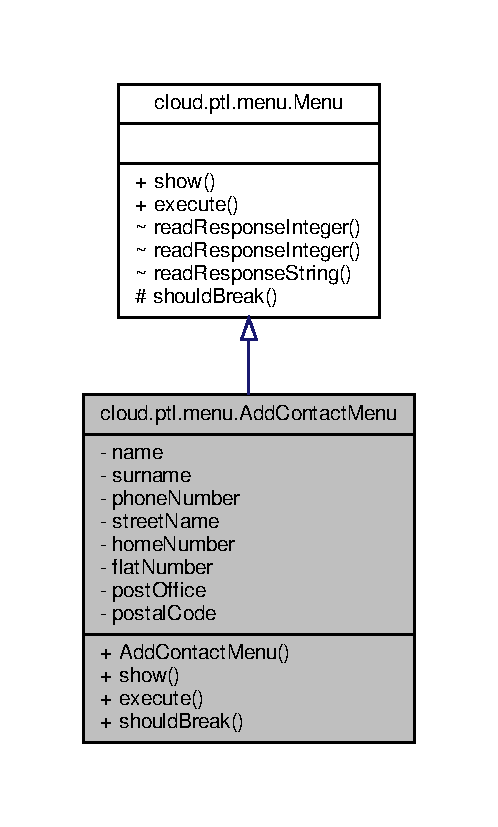
\includegraphics[width=239pt]{classcloud_1_1ptl_1_1menu_1_1AddContactMenu__inherit__graph}
\end{center}
\end{figure}


Collaboration diagram for cloud.\+ptl.\+menu.\+Add\+Contact\+Menu\+:
\nopagebreak
\begin{figure}[H]
\begin{center}
\leavevmode
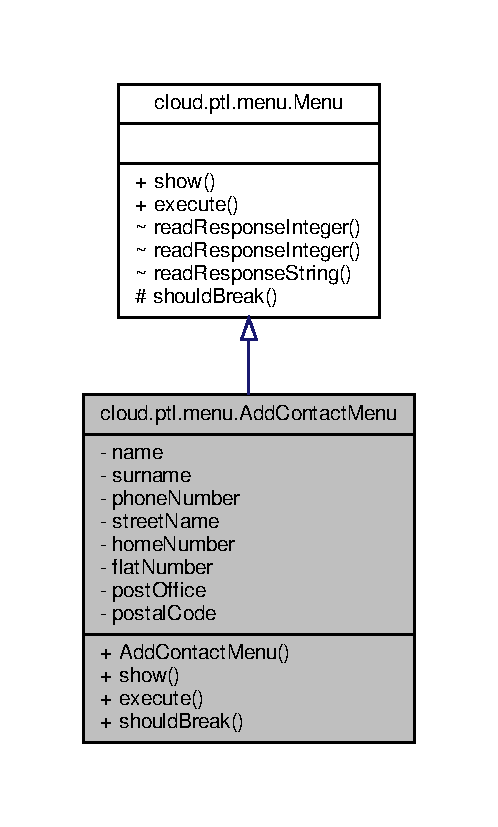
\includegraphics[width=239pt]{classcloud_1_1ptl_1_1menu_1_1AddContactMenu__coll__graph}
\end{center}
\end{figure}
\subsection*{Public Member Functions}
\begin{DoxyCompactItemize}
\item 
\mbox{\Hypertarget{classcloud_1_1ptl_1_1menu_1_1AddContactMenu_a4a777d242c4272af84d36d59ebfd5780}\label{classcloud_1_1ptl_1_1menu_1_1AddContactMenu_a4a777d242c4272af84d36d59ebfd5780}} 
void {\bfseries show} ()
\item 
\mbox{\Hypertarget{classcloud_1_1ptl_1_1menu_1_1AddContactMenu_a558adf8fececd6a2afe43b3415e46418}\label{classcloud_1_1ptl_1_1menu_1_1AddContactMenu_a558adf8fececd6a2afe43b3415e46418}} 
void {\bfseries execute} ()
\item 
\mbox{\Hypertarget{classcloud_1_1ptl_1_1menu_1_1AddContactMenu_ac712784ee8666bc60a6818492aff600c}\label{classcloud_1_1ptl_1_1menu_1_1AddContactMenu_ac712784ee8666bc60a6818492aff600c}} 
Boolean {\bfseries should\+Break} ()
\end{DoxyCompactItemize}
\subsection*{Private Attributes}
\begin{DoxyCompactItemize}
\item 
\mbox{\Hypertarget{classcloud_1_1ptl_1_1menu_1_1AddContactMenu_a4100893769d7b252bd944354a83108fa}\label{classcloud_1_1ptl_1_1menu_1_1AddContactMenu_a4100893769d7b252bd944354a83108fa}} 
String {\bfseries name}
\item 
\mbox{\Hypertarget{classcloud_1_1ptl_1_1menu_1_1AddContactMenu_ad6e860278ebf81977ccf91e3f47e5f7e}\label{classcloud_1_1ptl_1_1menu_1_1AddContactMenu_ad6e860278ebf81977ccf91e3f47e5f7e}} 
String {\bfseries surname}
\item 
\mbox{\Hypertarget{classcloud_1_1ptl_1_1menu_1_1AddContactMenu_a66730bc98b7350577f1f4078fb3936f2}\label{classcloud_1_1ptl_1_1menu_1_1AddContactMenu_a66730bc98b7350577f1f4078fb3936f2}} 
String {\bfseries phone\+Number}
\item 
\mbox{\Hypertarget{classcloud_1_1ptl_1_1menu_1_1AddContactMenu_a23a1c4f99d2e59b068c67403b23072bc}\label{classcloud_1_1ptl_1_1menu_1_1AddContactMenu_a23a1c4f99d2e59b068c67403b23072bc}} 
String {\bfseries street\+Name}
\item 
\mbox{\Hypertarget{classcloud_1_1ptl_1_1menu_1_1AddContactMenu_af3a2d2e905dbbdaae261c5c62dd188ec}\label{classcloud_1_1ptl_1_1menu_1_1AddContactMenu_af3a2d2e905dbbdaae261c5c62dd188ec}} 
Integer {\bfseries home\+Number}
\item 
\mbox{\Hypertarget{classcloud_1_1ptl_1_1menu_1_1AddContactMenu_a9cda1b0ee5818217482df7bc5bb2bff9}\label{classcloud_1_1ptl_1_1menu_1_1AddContactMenu_a9cda1b0ee5818217482df7bc5bb2bff9}} 
Integer {\bfseries flat\+Number}
\item 
\mbox{\Hypertarget{classcloud_1_1ptl_1_1menu_1_1AddContactMenu_aa8aed7909abeaa3b52ae565e7c84404f}\label{classcloud_1_1ptl_1_1menu_1_1AddContactMenu_aa8aed7909abeaa3b52ae565e7c84404f}} 
String {\bfseries post\+Office}
\item 
\mbox{\Hypertarget{classcloud_1_1ptl_1_1menu_1_1AddContactMenu_a62f5dd68381973485600264d5c0061cf}\label{classcloud_1_1ptl_1_1menu_1_1AddContactMenu_a62f5dd68381973485600264d5c0061cf}} 
String {\bfseries postal\+Code}
\end{DoxyCompactItemize}
\subsection*{Additional Inherited Members}


The documentation for this class was generated from the following file\+:\begin{DoxyCompactItemize}
\item 
src/main/java/cloud/ptl/menu/Add\+Contact\+Menu.\+java\end{DoxyCompactItemize}

\hypertarget{classcloud_1_1ptl_1_1persistence_1_1Address}{}\section{cloud.\+ptl.\+persistence.\+Address Class Reference}
\label{classcloud_1_1ptl_1_1persistence_1_1Address}\index{cloud.\+ptl.\+persistence.\+Address@{cloud.\+ptl.\+persistence.\+Address}}


Inheritance diagram for cloud.\+ptl.\+persistence.\+Address\+:
\nopagebreak
\begin{figure}[H]
\begin{center}
\leavevmode
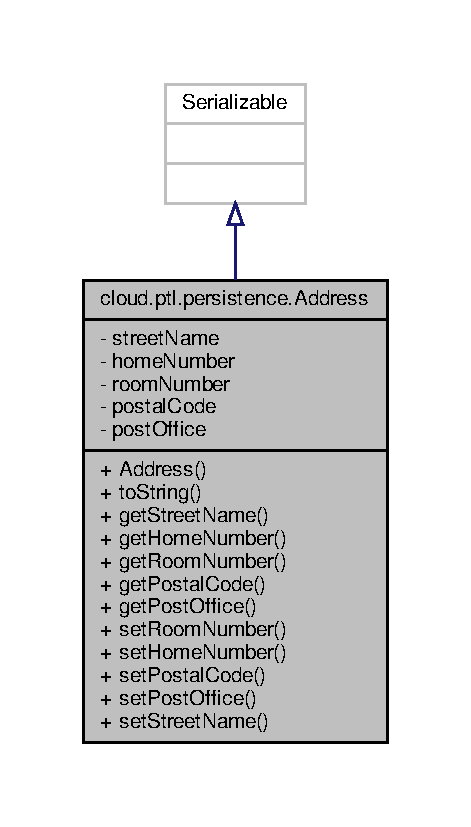
\includegraphics[width=226pt]{classcloud_1_1ptl_1_1persistence_1_1Address__inherit__graph}
\end{center}
\end{figure}


Collaboration diagram for cloud.\+ptl.\+persistence.\+Address\+:
\nopagebreak
\begin{figure}[H]
\begin{center}
\leavevmode
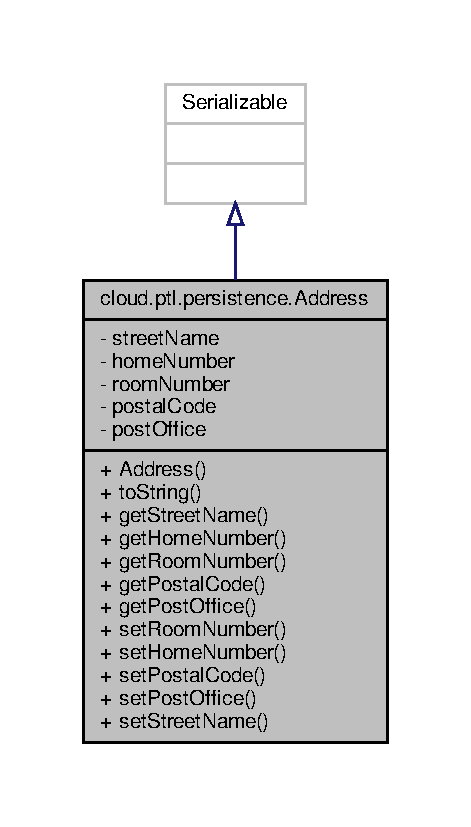
\includegraphics[width=226pt]{classcloud_1_1ptl_1_1persistence_1_1Address__coll__graph}
\end{center}
\end{figure}
\subsection*{Public Member Functions}
\begin{DoxyCompactItemize}
\item 
\mbox{\Hypertarget{classcloud_1_1ptl_1_1persistence_1_1Address_ad83591046735ac0e7d88ca1da8a89d8c}\label{classcloud_1_1ptl_1_1persistence_1_1Address_ad83591046735ac0e7d88ca1da8a89d8c}} 
{\bfseries Address} (String street\+Name, Integer home\+Number, Integer room\+Number, String postal\+Code, String post\+Office)
\item 
\mbox{\Hypertarget{classcloud_1_1ptl_1_1persistence_1_1Address_a2aefc513b9af1a2dc576c3cbd099370a}\label{classcloud_1_1ptl_1_1persistence_1_1Address_a2aefc513b9af1a2dc576c3cbd099370a}} 
String {\bfseries to\+String} ()
\item 
\mbox{\Hypertarget{classcloud_1_1ptl_1_1persistence_1_1Address_a8d0b0b9e58efb70f6d87f388b1b99128}\label{classcloud_1_1ptl_1_1persistence_1_1Address_a8d0b0b9e58efb70f6d87f388b1b99128}} 
String {\bfseries get\+Street\+Name} ()
\item 
\mbox{\Hypertarget{classcloud_1_1ptl_1_1persistence_1_1Address_abdd09a9a589a3626e5ae9d9b55ee0eb6}\label{classcloud_1_1ptl_1_1persistence_1_1Address_abdd09a9a589a3626e5ae9d9b55ee0eb6}} 
Integer {\bfseries get\+Home\+Number} ()
\item 
\mbox{\Hypertarget{classcloud_1_1ptl_1_1persistence_1_1Address_a259fd5d466d576c6f5fd3693d0f54db3}\label{classcloud_1_1ptl_1_1persistence_1_1Address_a259fd5d466d576c6f5fd3693d0f54db3}} 
Integer {\bfseries get\+Room\+Number} ()
\item 
\mbox{\Hypertarget{classcloud_1_1ptl_1_1persistence_1_1Address_a8b5cfda35d887e7e0c102266a7d0826a}\label{classcloud_1_1ptl_1_1persistence_1_1Address_a8b5cfda35d887e7e0c102266a7d0826a}} 
String {\bfseries get\+Postal\+Code} ()
\item 
\mbox{\Hypertarget{classcloud_1_1ptl_1_1persistence_1_1Address_ae85b0f9a9ed1044c3e38178bc3c9b25d}\label{classcloud_1_1ptl_1_1persistence_1_1Address_ae85b0f9a9ed1044c3e38178bc3c9b25d}} 
String {\bfseries get\+Post\+Office} ()
\item 
\mbox{\Hypertarget{classcloud_1_1ptl_1_1persistence_1_1Address_ad3e64b1830118ca85d013d4dbd1d8b12}\label{classcloud_1_1ptl_1_1persistence_1_1Address_ad3e64b1830118ca85d013d4dbd1d8b12}} 
void {\bfseries set\+Room\+Number} (Integer room\+Number)
\item 
\mbox{\Hypertarget{classcloud_1_1ptl_1_1persistence_1_1Address_a8e25fa83c670ff8143823277a91b0d12}\label{classcloud_1_1ptl_1_1persistence_1_1Address_a8e25fa83c670ff8143823277a91b0d12}} 
void {\bfseries set\+Home\+Number} (Integer home\+Number)
\item 
\mbox{\Hypertarget{classcloud_1_1ptl_1_1persistence_1_1Address_a3a51d4921cd04b37e501d8a909e2ffbb}\label{classcloud_1_1ptl_1_1persistence_1_1Address_a3a51d4921cd04b37e501d8a909e2ffbb}} 
void {\bfseries set\+Postal\+Code} (String postal\+Code)
\item 
\mbox{\Hypertarget{classcloud_1_1ptl_1_1persistence_1_1Address_a02e3d1af0fb3d62ba5fe1478f9e02d74}\label{classcloud_1_1ptl_1_1persistence_1_1Address_a02e3d1af0fb3d62ba5fe1478f9e02d74}} 
void {\bfseries set\+Post\+Office} (String post\+Office)
\item 
\mbox{\Hypertarget{classcloud_1_1ptl_1_1persistence_1_1Address_ae6837d17b8e5b78e81ace9e08e7a648e}\label{classcloud_1_1ptl_1_1persistence_1_1Address_ae6837d17b8e5b78e81ace9e08e7a648e}} 
void {\bfseries set\+Street\+Name} (String street\+Name)
\end{DoxyCompactItemize}
\subsection*{Private Attributes}
\begin{DoxyCompactItemize}
\item 
\mbox{\Hypertarget{classcloud_1_1ptl_1_1persistence_1_1Address_a77469e220f9c70512deb596be619371b}\label{classcloud_1_1ptl_1_1persistence_1_1Address_a77469e220f9c70512deb596be619371b}} 
String {\bfseries street\+Name}
\item 
\mbox{\Hypertarget{classcloud_1_1ptl_1_1persistence_1_1Address_a24180fd7276a5d82860a3e3451356095}\label{classcloud_1_1ptl_1_1persistence_1_1Address_a24180fd7276a5d82860a3e3451356095}} 
Integer {\bfseries home\+Number}
\item 
\mbox{\Hypertarget{classcloud_1_1ptl_1_1persistence_1_1Address_a56795b86edf1fa64f90a903102f5e572}\label{classcloud_1_1ptl_1_1persistence_1_1Address_a56795b86edf1fa64f90a903102f5e572}} 
Integer {\bfseries room\+Number}
\item 
\mbox{\Hypertarget{classcloud_1_1ptl_1_1persistence_1_1Address_af10b444d134b57e130f4bdf9fc4b0065}\label{classcloud_1_1ptl_1_1persistence_1_1Address_af10b444d134b57e130f4bdf9fc4b0065}} 
String {\bfseries postal\+Code}
\item 
\mbox{\Hypertarget{classcloud_1_1ptl_1_1persistence_1_1Address_a5606e0bd6c390bc1f562ac8db4661a3a}\label{classcloud_1_1ptl_1_1persistence_1_1Address_a5606e0bd6c390bc1f562ac8db4661a3a}} 
String {\bfseries post\+Office}
\end{DoxyCompactItemize}


The documentation for this class was generated from the following file\+:\begin{DoxyCompactItemize}
\item 
src/main/java/cloud/ptl/persistence/Address.\+java\end{DoxyCompactItemize}

\hypertarget{classcloud_1_1ptl_1_1App}{}\section{cloud.\+ptl.\+App Class Reference}
\label{classcloud_1_1ptl_1_1App}\index{cloud.\+ptl.\+App@{cloud.\+ptl.\+App}}


Collaboration diagram for cloud.\+ptl.\+App\+:
\nopagebreak
\begin{figure}[H]
\begin{center}
\leavevmode
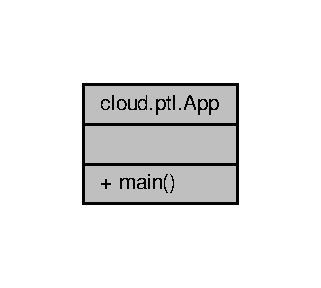
\includegraphics[width=154pt]{classcloud_1_1ptl_1_1App__coll__graph}
\end{center}
\end{figure}
\subsection*{Static Public Member Functions}
\begin{DoxyCompactItemize}
\item 
\mbox{\Hypertarget{classcloud_1_1ptl_1_1App_ace8b2eb7c056f71d94d91f150d976319}\label{classcloud_1_1ptl_1_1App_ace8b2eb7c056f71d94d91f150d976319}} 
static void {\bfseries main} (String\mbox{[}$\,$\mbox{]} args)
\end{DoxyCompactItemize}


\subsection{Detailed Description}
Hello world! 

The documentation for this class was generated from the following file\+:\begin{DoxyCompactItemize}
\item 
src/main/java/cloud/ptl/App.\+java\end{DoxyCompactItemize}

\hypertarget{classcloud_1_1ptl_1_1AppTest}{}\section{cloud.\+ptl.\+App\+Test Class Reference}
\label{classcloud_1_1ptl_1_1AppTest}\index{cloud.\+ptl.\+App\+Test@{cloud.\+ptl.\+App\+Test}}


Collaboration diagram for cloud.\+ptl.\+App\+Test\+:
\nopagebreak
\begin{figure}[H]
\begin{center}
\leavevmode
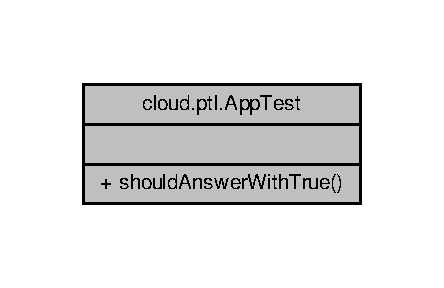
\includegraphics[width=213pt]{classcloud_1_1ptl_1_1AppTest__coll__graph}
\end{center}
\end{figure}
\subsection*{Public Member Functions}
\begin{DoxyCompactItemize}
\item 
void \hyperlink{classcloud_1_1ptl_1_1AppTest_ad4615d98b5e2e065cc330ed6eb6a33c7}{should\+Answer\+With\+True} ()
\end{DoxyCompactItemize}


\subsection{Detailed Description}
Unit test for simple \hyperlink{classcloud_1_1ptl_1_1App}{App}. 

\subsection{Member Function Documentation}
\mbox{\Hypertarget{classcloud_1_1ptl_1_1AppTest_ad4615d98b5e2e065cc330ed6eb6a33c7}\label{classcloud_1_1ptl_1_1AppTest_ad4615d98b5e2e065cc330ed6eb6a33c7}} 
\index{cloud\+::ptl\+::\+App\+Test@{cloud\+::ptl\+::\+App\+Test}!should\+Answer\+With\+True@{should\+Answer\+With\+True}}
\index{should\+Answer\+With\+True@{should\+Answer\+With\+True}!cloud\+::ptl\+::\+App\+Test@{cloud\+::ptl\+::\+App\+Test}}
\subsubsection{\texorpdfstring{should\+Answer\+With\+True()}{shouldAnswerWithTrue()}}
{\footnotesize\ttfamily void cloud.\+ptl.\+App\+Test.\+should\+Answer\+With\+True (\begin{DoxyParamCaption}{ }\end{DoxyParamCaption})\hspace{0.3cm}{\ttfamily [inline]}}

Rigorous Test \+:-\/) 

The documentation for this class was generated from the following file\+:\begin{DoxyCompactItemize}
\item 
src/test/java/cloud/ptl/App\+Test.\+java\end{DoxyCompactItemize}

\hypertarget{classcloud_1_1ptl_1_1persistence_1_1Contact}{}\section{cloud.\+ptl.\+persistence.\+Contact Class Reference}
\label{classcloud_1_1ptl_1_1persistence_1_1Contact}\index{cloud.\+ptl.\+persistence.\+Contact@{cloud.\+ptl.\+persistence.\+Contact}}


Inheritance diagram for cloud.\+ptl.\+persistence.\+Contact\+:
\nopagebreak
\begin{figure}[H]
\begin{center}
\leavevmode
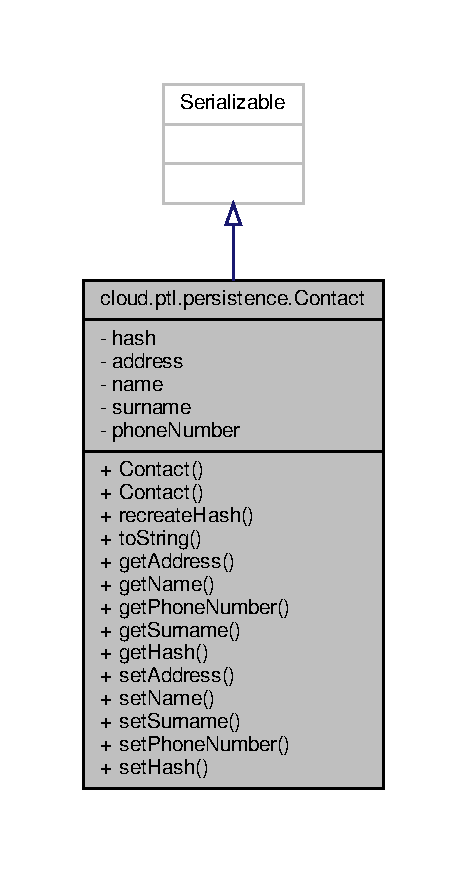
\includegraphics[width=224pt]{classcloud_1_1ptl_1_1persistence_1_1Contact__inherit__graph}
\end{center}
\end{figure}


Collaboration diagram for cloud.\+ptl.\+persistence.\+Contact\+:
\nopagebreak
\begin{figure}[H]
\begin{center}
\leavevmode
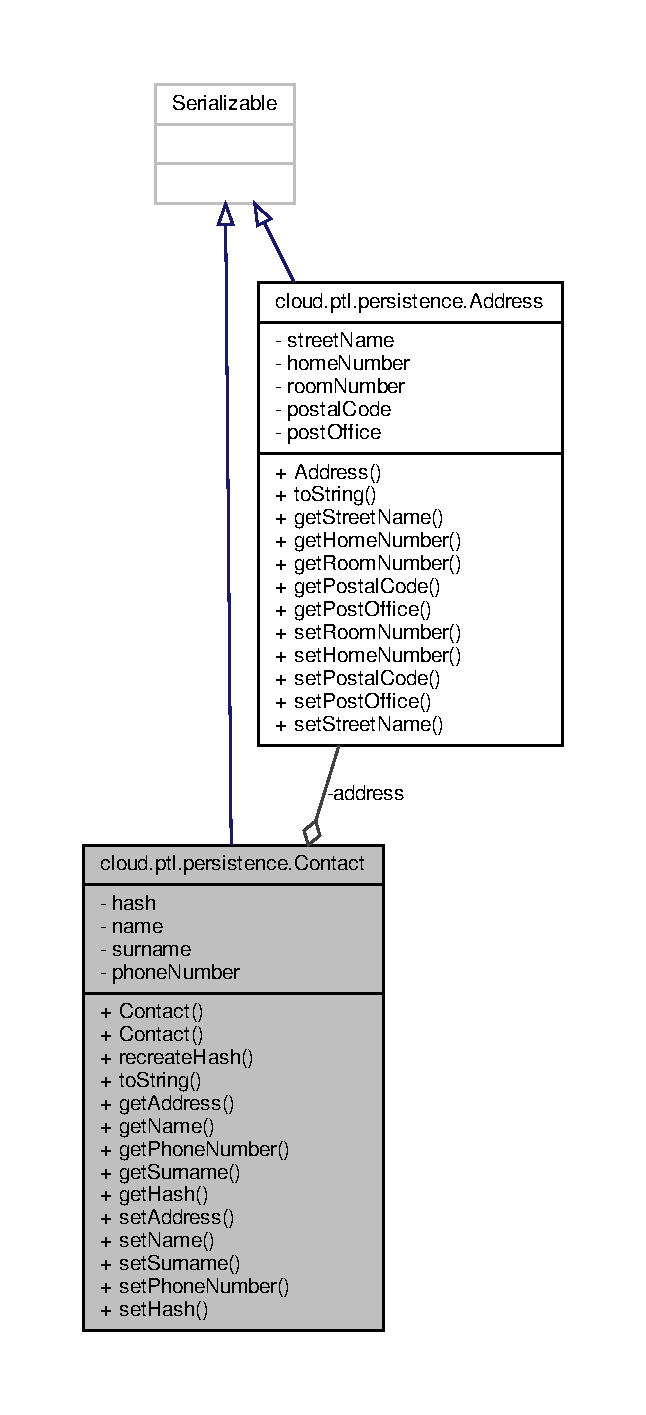
\includegraphics[height=550pt]{classcloud_1_1ptl_1_1persistence_1_1Contact__coll__graph}
\end{center}
\end{figure}
\subsection*{Public Member Functions}
\begin{DoxyCompactItemize}
\item 
\mbox{\Hypertarget{classcloud_1_1ptl_1_1persistence_1_1Contact_a9632e36b8155c5904e15ebf88a63319f}\label{classcloud_1_1ptl_1_1persistence_1_1Contact_a9632e36b8155c5904e15ebf88a63319f}} 
{\bfseries Contact} (String name, String surname, String phone\+Number, \hyperlink{classcloud_1_1ptl_1_1persistence_1_1Address}{Address} address)
\item 
\mbox{\Hypertarget{classcloud_1_1ptl_1_1persistence_1_1Contact_af936a2f94db71920c6c8cf52bc43af8c}\label{classcloud_1_1ptl_1_1persistence_1_1Contact_af936a2f94db71920c6c8cf52bc43af8c}} 
void {\bfseries recreate\+Hash} ()
\item 
\mbox{\Hypertarget{classcloud_1_1ptl_1_1persistence_1_1Contact_a8e0732a83078d44c615ecc4740f50a76}\label{classcloud_1_1ptl_1_1persistence_1_1Contact_a8e0732a83078d44c615ecc4740f50a76}} 
String {\bfseries to\+String} ()
\item 
\mbox{\Hypertarget{classcloud_1_1ptl_1_1persistence_1_1Contact_afc86bebcb1976b7ee21adb71dbacb7da}\label{classcloud_1_1ptl_1_1persistence_1_1Contact_afc86bebcb1976b7ee21adb71dbacb7da}} 
\hyperlink{classcloud_1_1ptl_1_1persistence_1_1Address}{Address} {\bfseries get\+Address} ()
\item 
\mbox{\Hypertarget{classcloud_1_1ptl_1_1persistence_1_1Contact_a993d57bf28a4a2af65783a06ecb1db8e}\label{classcloud_1_1ptl_1_1persistence_1_1Contact_a993d57bf28a4a2af65783a06ecb1db8e}} 
String {\bfseries get\+Name} ()
\item 
\mbox{\Hypertarget{classcloud_1_1ptl_1_1persistence_1_1Contact_a9a599f3cb99c9cc02ff4fbc461e990c0}\label{classcloud_1_1ptl_1_1persistence_1_1Contact_a9a599f3cb99c9cc02ff4fbc461e990c0}} 
String {\bfseries get\+Phone\+Number} ()
\item 
\mbox{\Hypertarget{classcloud_1_1ptl_1_1persistence_1_1Contact_a0900199420419f679736980a90e87a6b}\label{classcloud_1_1ptl_1_1persistence_1_1Contact_a0900199420419f679736980a90e87a6b}} 
String {\bfseries get\+Surname} ()
\item 
\mbox{\Hypertarget{classcloud_1_1ptl_1_1persistence_1_1Contact_ae44a8c27686466703874c0654be883a9}\label{classcloud_1_1ptl_1_1persistence_1_1Contact_ae44a8c27686466703874c0654be883a9}} 
String {\bfseries get\+Hash} ()
\item 
\mbox{\Hypertarget{classcloud_1_1ptl_1_1persistence_1_1Contact_a5678d9b0baf9a769dbd1ef55a1c34a06}\label{classcloud_1_1ptl_1_1persistence_1_1Contact_a5678d9b0baf9a769dbd1ef55a1c34a06}} 
void {\bfseries set\+Address} (\hyperlink{classcloud_1_1ptl_1_1persistence_1_1Address}{Address} address)
\item 
\mbox{\Hypertarget{classcloud_1_1ptl_1_1persistence_1_1Contact_a849698b63816e6d1c8dc682f0384732f}\label{classcloud_1_1ptl_1_1persistence_1_1Contact_a849698b63816e6d1c8dc682f0384732f}} 
void {\bfseries set\+Name} (String name)
\item 
\mbox{\Hypertarget{classcloud_1_1ptl_1_1persistence_1_1Contact_ac72e996bcc5d125ffd9a07874b39be44}\label{classcloud_1_1ptl_1_1persistence_1_1Contact_ac72e996bcc5d125ffd9a07874b39be44}} 
void {\bfseries set\+Surname} (String surname)
\item 
\mbox{\Hypertarget{classcloud_1_1ptl_1_1persistence_1_1Contact_a5547e57c669f1a6de9691a1ab47d5f26}\label{classcloud_1_1ptl_1_1persistence_1_1Contact_a5547e57c669f1a6de9691a1ab47d5f26}} 
void {\bfseries set\+Phone\+Number} (String phone\+Number)
\item 
\mbox{\Hypertarget{classcloud_1_1ptl_1_1persistence_1_1Contact_ac1d4a228747fb867e2773f7c020a9cbe}\label{classcloud_1_1ptl_1_1persistence_1_1Contact_ac1d4a228747fb867e2773f7c020a9cbe}} 
void {\bfseries set\+Hash} (String hash)
\end{DoxyCompactItemize}
\subsection*{Private Attributes}
\begin{DoxyCompactItemize}
\item 
\mbox{\Hypertarget{classcloud_1_1ptl_1_1persistence_1_1Contact_a38119a4d669f08b70046184cddb93c53}\label{classcloud_1_1ptl_1_1persistence_1_1Contact_a38119a4d669f08b70046184cddb93c53}} 
String {\bfseries hash}
\item 
\mbox{\Hypertarget{classcloud_1_1ptl_1_1persistence_1_1Contact_abdfad8c1a96dc90f995763c9a219125d}\label{classcloud_1_1ptl_1_1persistence_1_1Contact_abdfad8c1a96dc90f995763c9a219125d}} 
\hyperlink{classcloud_1_1ptl_1_1persistence_1_1Address}{Address} {\bfseries address}
\item 
\mbox{\Hypertarget{classcloud_1_1ptl_1_1persistence_1_1Contact_a752a428438ac61bca2f7f48f541a4d63}\label{classcloud_1_1ptl_1_1persistence_1_1Contact_a752a428438ac61bca2f7f48f541a4d63}} 
String {\bfseries name}
\item 
\mbox{\Hypertarget{classcloud_1_1ptl_1_1persistence_1_1Contact_aab338712c38ce4412e274d56f41de3aa}\label{classcloud_1_1ptl_1_1persistence_1_1Contact_aab338712c38ce4412e274d56f41de3aa}} 
String {\bfseries surname}
\item 
\mbox{\Hypertarget{classcloud_1_1ptl_1_1persistence_1_1Contact_a62fb5cb4f6117cb8e568b4ff4094f33b}\label{classcloud_1_1ptl_1_1persistence_1_1Contact_a62fb5cb4f6117cb8e568b4ff4094f33b}} 
String {\bfseries phone\+Number}
\end{DoxyCompactItemize}


The documentation for this class was generated from the following file\+:\begin{DoxyCompactItemize}
\item 
src/main/java/cloud/ptl/persistence/Contact.\+java\end{DoxyCompactItemize}

\hypertarget{enumcloud_1_1ptl_1_1persistence_1_1ContactFields}{}\section{cloud.\+ptl.\+persistence.\+Contact\+Fields Enum Reference}
\label{enumcloud_1_1ptl_1_1persistence_1_1ContactFields}\index{cloud.\+ptl.\+persistence.\+Contact\+Fields@{cloud.\+ptl.\+persistence.\+Contact\+Fields}}


Collaboration diagram for cloud.\+ptl.\+persistence.\+Contact\+Fields\+:
\nopagebreak
\begin{figure}[H]
\begin{center}
\leavevmode
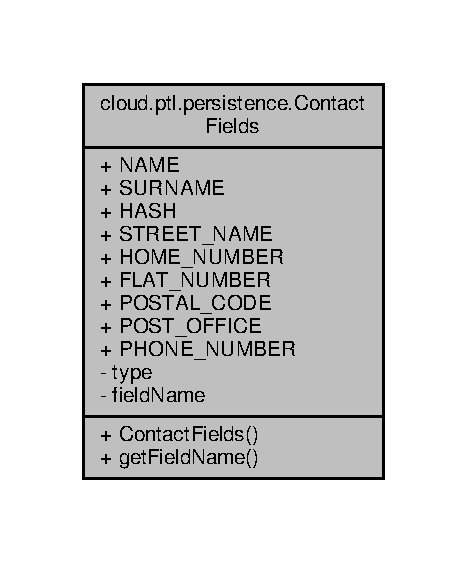
\includegraphics[width=224pt]{enumcloud_1_1ptl_1_1persistence_1_1ContactFields__coll__graph}
\end{center}
\end{figure}
\subsection*{Public Member Functions}
\begin{DoxyCompactItemize}
\item 
\mbox{\Hypertarget{enumcloud_1_1ptl_1_1persistence_1_1ContactFields_ae64d692f1ab9f31b752f901075d3e7b8}\label{enumcloud_1_1ptl_1_1persistence_1_1ContactFields_ae64d692f1ab9f31b752f901075d3e7b8}} 
{\bfseries Contact\+Fields} (String type, String field\+Name)
\item 
\mbox{\Hypertarget{enumcloud_1_1ptl_1_1persistence_1_1ContactFields_ab08b7b43a8aedb74b26be8de52087a20}\label{enumcloud_1_1ptl_1_1persistence_1_1ContactFields_ab08b7b43a8aedb74b26be8de52087a20}} 
String {\bfseries get\+Field\+Name} ()
\end{DoxyCompactItemize}
\subsection*{Public Attributes}
\begin{DoxyCompactItemize}
\item 
\mbox{\Hypertarget{enumcloud_1_1ptl_1_1persistence_1_1ContactFields_a60ca1f5df4addfa41076dbf209f51712}\label{enumcloud_1_1ptl_1_1persistence_1_1ContactFields_a60ca1f5df4addfa41076dbf209f51712}} 
{\bfseries N\+A\+ME} =(\char`\"{}String\char`\"{}, \char`\"{}Name\char`\"{})
\item 
\mbox{\Hypertarget{enumcloud_1_1ptl_1_1persistence_1_1ContactFields_a735ef02829ae3bc1523762b9293afe87}\label{enumcloud_1_1ptl_1_1persistence_1_1ContactFields_a735ef02829ae3bc1523762b9293afe87}} 
{\bfseries S\+U\+R\+N\+A\+ME} =(\char`\"{}String\char`\"{}, \char`\"{}Surname\char`\"{})
\item 
\mbox{\Hypertarget{enumcloud_1_1ptl_1_1persistence_1_1ContactFields_ac8e9fb5cc6eca997143fe320bd5288d9}\label{enumcloud_1_1ptl_1_1persistence_1_1ContactFields_ac8e9fb5cc6eca997143fe320bd5288d9}} 
{\bfseries H\+A\+SH} =(\char`\"{}String\char`\"{}, \char`\"{}Hash\char`\"{})
\item 
\mbox{\Hypertarget{enumcloud_1_1ptl_1_1persistence_1_1ContactFields_a3c4b93237f421a53fbc0154136a7b9c1}\label{enumcloud_1_1ptl_1_1persistence_1_1ContactFields_a3c4b93237f421a53fbc0154136a7b9c1}} 
{\bfseries S\+T\+R\+E\+E\+T\+\_\+\+N\+A\+ME} =(\char`\"{}String\char`\"{}, \char`\"{}Street\+\_\+\+Name\char`\"{})
\item 
\mbox{\Hypertarget{enumcloud_1_1ptl_1_1persistence_1_1ContactFields_a293dd59f16433313b9418679725f44fe}\label{enumcloud_1_1ptl_1_1persistence_1_1ContactFields_a293dd59f16433313b9418679725f44fe}} 
{\bfseries H\+O\+M\+E\+\_\+\+N\+U\+M\+B\+ER} =(\char`\"{}Integer\char`\"{}, \char`\"{}Home\+\_\+\+Number\char`\"{})
\item 
\mbox{\Hypertarget{enumcloud_1_1ptl_1_1persistence_1_1ContactFields_a1fc066f09c9c629761a9303ae205ccce}\label{enumcloud_1_1ptl_1_1persistence_1_1ContactFields_a1fc066f09c9c629761a9303ae205ccce}} 
{\bfseries F\+L\+A\+T\+\_\+\+N\+U\+M\+B\+ER} =(\char`\"{}Integer\char`\"{}, \char`\"{}Flat\+\_\+\+Number\char`\"{})
\item 
\mbox{\Hypertarget{enumcloud_1_1ptl_1_1persistence_1_1ContactFields_aa64b438cb983c67092cc0db341bc1910}\label{enumcloud_1_1ptl_1_1persistence_1_1ContactFields_aa64b438cb983c67092cc0db341bc1910}} 
{\bfseries P\+O\+S\+T\+A\+L\+\_\+\+C\+O\+DE} =(\char`\"{}String\char`\"{}, \char`\"{}Postal\+\_\+\+Code\char`\"{})
\item 
\mbox{\Hypertarget{enumcloud_1_1ptl_1_1persistence_1_1ContactFields_ac8c9e2a31552b474755f035e3654e7f1}\label{enumcloud_1_1ptl_1_1persistence_1_1ContactFields_ac8c9e2a31552b474755f035e3654e7f1}} 
{\bfseries P\+O\+S\+T\+\_\+\+O\+F\+F\+I\+CE} =(\char`\"{}String\char`\"{}, \char`\"{}Post\+\_\+\+Office\char`\"{})
\item 
\mbox{\Hypertarget{enumcloud_1_1ptl_1_1persistence_1_1ContactFields_ae35985bb3fcd017c8812e4c2f2a28bd6}\label{enumcloud_1_1ptl_1_1persistence_1_1ContactFields_ae35985bb3fcd017c8812e4c2f2a28bd6}} 
{\bfseries P\+H\+O\+N\+E\+\_\+\+N\+U\+M\+B\+ER} =(\char`\"{}String\char`\"{}, \char`\"{}Phone\+\_\+\+Number\char`\"{})
\end{DoxyCompactItemize}
\subsection*{Private Attributes}
\begin{DoxyCompactItemize}
\item 
\mbox{\Hypertarget{enumcloud_1_1ptl_1_1persistence_1_1ContactFields_af6f681a44a0c774b195a29a8b02eff20}\label{enumcloud_1_1ptl_1_1persistence_1_1ContactFields_af6f681a44a0c774b195a29a8b02eff20}} 
final String {\bfseries type}
\item 
\mbox{\Hypertarget{enumcloud_1_1ptl_1_1persistence_1_1ContactFields_a275aff30051cb54b3cdda806632ff853}\label{enumcloud_1_1ptl_1_1persistence_1_1ContactFields_a275aff30051cb54b3cdda806632ff853}} 
final String {\bfseries field\+Name}
\end{DoxyCompactItemize}


The documentation for this enum was generated from the following file\+:\begin{DoxyCompactItemize}
\item 
src/main/java/cloud/ptl/persistence/Contact\+Fields.\+java\end{DoxyCompactItemize}

\hypertarget{classcloud_1_1ptl_1_1persistence_1_1ContactManager}{}\section{cloud.\+ptl.\+persistence.\+Contact\+Manager Class Reference}
\label{classcloud_1_1ptl_1_1persistence_1_1ContactManager}\index{cloud.\+ptl.\+persistence.\+Contact\+Manager@{cloud.\+ptl.\+persistence.\+Contact\+Manager}}


Collaboration diagram for cloud.\+ptl.\+persistence.\+Contact\+Manager\+:
\nopagebreak
\begin{figure}[H]
\begin{center}
\leavevmode
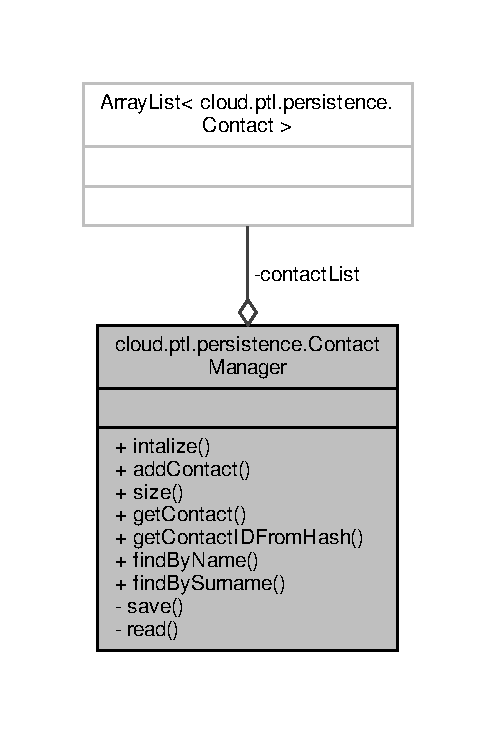
\includegraphics[width=238pt]{classcloud_1_1ptl_1_1persistence_1_1ContactManager__coll__graph}
\end{center}
\end{figure}
\subsection*{Static Public Member Functions}
\begin{DoxyCompactItemize}
\item 
\mbox{\Hypertarget{classcloud_1_1ptl_1_1persistence_1_1ContactManager_ab7b470e606d49db74c139adbcceeb782}\label{classcloud_1_1ptl_1_1persistence_1_1ContactManager_ab7b470e606d49db74c139adbcceeb782}} 
static void {\bfseries intalize} ()
\item 
\mbox{\Hypertarget{classcloud_1_1ptl_1_1persistence_1_1ContactManager_a09926dcf77240781f05e4157ef365658}\label{classcloud_1_1ptl_1_1persistence_1_1ContactManager_a09926dcf77240781f05e4157ef365658}} 
static void {\bfseries add\+Contact} (\hyperlink{classcloud_1_1ptl_1_1persistence_1_1Contact}{Contact} new\+Contact)
\item 
\mbox{\Hypertarget{classcloud_1_1ptl_1_1persistence_1_1ContactManager_ade1723d6dbbaa5eff75aa83fa761d2ac}\label{classcloud_1_1ptl_1_1persistence_1_1ContactManager_ade1723d6dbbaa5eff75aa83fa761d2ac}} 
static Integer {\bfseries size} ()
\item 
\mbox{\Hypertarget{classcloud_1_1ptl_1_1persistence_1_1ContactManager_a5817e662f7568040b24dea9151ff2340}\label{classcloud_1_1ptl_1_1persistence_1_1ContactManager_a5817e662f7568040b24dea9151ff2340}} 
static \hyperlink{classcloud_1_1ptl_1_1persistence_1_1Contact}{Contact} {\bfseries get\+Contact} (int position)
\item 
\mbox{\Hypertarget{classcloud_1_1ptl_1_1persistence_1_1ContactManager_af214473ac147cefe2435594e81471b81}\label{classcloud_1_1ptl_1_1persistence_1_1ContactManager_af214473ac147cefe2435594e81471b81}} 
static Integer {\bfseries get\+Contact\+I\+D\+From\+Hash} (String hash)
\item 
\mbox{\Hypertarget{classcloud_1_1ptl_1_1persistence_1_1ContactManager_a78f6913405f16e3f132307d92a0c4dc7}\label{classcloud_1_1ptl_1_1persistence_1_1ContactManager_a78f6913405f16e3f132307d92a0c4dc7}} 
static Array\+List$<$ \hyperlink{classcloud_1_1ptl_1_1persistence_1_1Contact}{Contact} $>$ {\bfseries find\+By\+Name} (String name)
\item 
\mbox{\Hypertarget{classcloud_1_1ptl_1_1persistence_1_1ContactManager_afee00f141daa7e27dd3c81dc759ab147}\label{classcloud_1_1ptl_1_1persistence_1_1ContactManager_afee00f141daa7e27dd3c81dc759ab147}} 
static Array\+List$<$ \hyperlink{classcloud_1_1ptl_1_1persistence_1_1Contact}{Contact} $>$ {\bfseries find\+By\+Surname} (String surname)
\end{DoxyCompactItemize}
\subsection*{Static Private Member Functions}
\begin{DoxyCompactItemize}
\item 
\mbox{\Hypertarget{classcloud_1_1ptl_1_1persistence_1_1ContactManager_a355c2df57a31d2e4c7dc42d697d64c50}\label{classcloud_1_1ptl_1_1persistence_1_1ContactManager_a355c2df57a31d2e4c7dc42d697d64c50}} 
static void {\bfseries save} ()
\item 
\mbox{\Hypertarget{classcloud_1_1ptl_1_1persistence_1_1ContactManager_a4c1f68a230573a4f2842139b46e3c8d9}\label{classcloud_1_1ptl_1_1persistence_1_1ContactManager_a4c1f68a230573a4f2842139b46e3c8d9}} 
static void {\bfseries read} ()
\end{DoxyCompactItemize}
\subsection*{Static Private Attributes}
\begin{DoxyCompactItemize}
\item 
\mbox{\Hypertarget{classcloud_1_1ptl_1_1persistence_1_1ContactManager_a6d025a6c5e6db2c3cae3df59056b94e7}\label{classcloud_1_1ptl_1_1persistence_1_1ContactManager_a6d025a6c5e6db2c3cae3df59056b94e7}} 
static Array\+List$<$ \hyperlink{classcloud_1_1ptl_1_1persistence_1_1Contact}{Contact} $>$ {\bfseries contact\+List}
\end{DoxyCompactItemize}


The documentation for this class was generated from the following file\+:\begin{DoxyCompactItemize}
\item 
src/main/java/cloud/ptl/persistence/Contact\+Manager.\+java\end{DoxyCompactItemize}

\hypertarget{classcloud_1_1ptl_1_1menu_1_1ContactSearchMenu}{}\section{cloud.\+ptl.\+menu.\+Contact\+Search\+Menu Class Reference}
\label{classcloud_1_1ptl_1_1menu_1_1ContactSearchMenu}\index{cloud.\+ptl.\+menu.\+Contact\+Search\+Menu@{cloud.\+ptl.\+menu.\+Contact\+Search\+Menu}}


Inheritance diagram for cloud.\+ptl.\+menu.\+Contact\+Search\+Menu\+:
\nopagebreak
\begin{figure}[H]
\begin{center}
\leavevmode
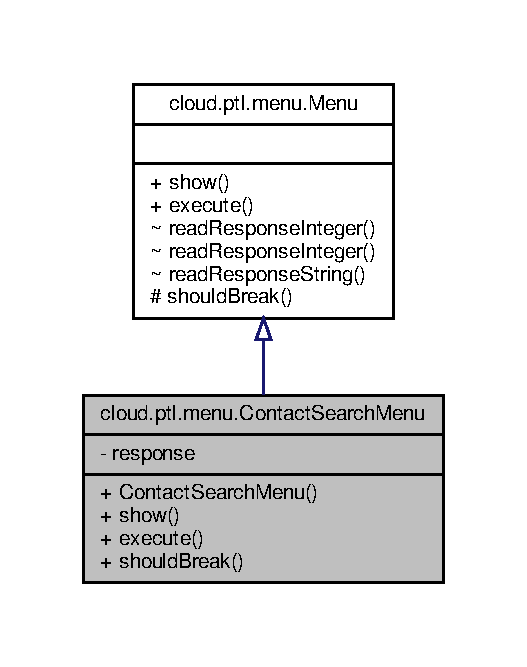
\includegraphics[width=253pt]{classcloud_1_1ptl_1_1menu_1_1ContactSearchMenu__inherit__graph}
\end{center}
\end{figure}


Collaboration diagram for cloud.\+ptl.\+menu.\+Contact\+Search\+Menu\+:
\nopagebreak
\begin{figure}[H]
\begin{center}
\leavevmode
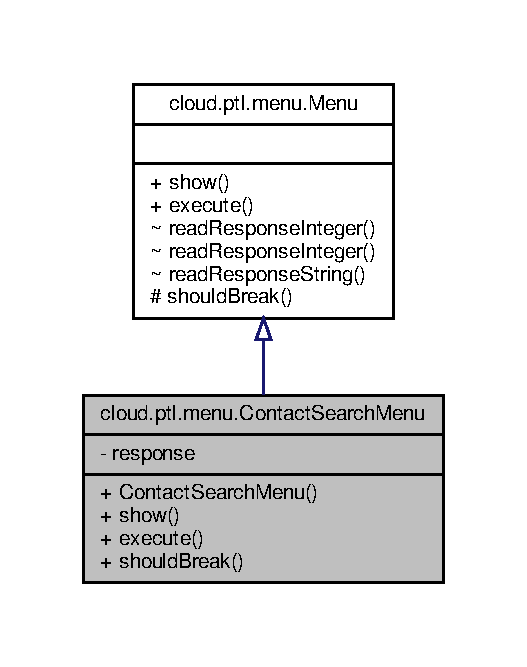
\includegraphics[width=253pt]{classcloud_1_1ptl_1_1menu_1_1ContactSearchMenu__coll__graph}
\end{center}
\end{figure}
\subsection*{Public Member Functions}
\begin{DoxyCompactItemize}
\item 
\mbox{\Hypertarget{classcloud_1_1ptl_1_1menu_1_1ContactSearchMenu_af6a25137b3e2d6a3a3ca8a3d19c71ff5}\label{classcloud_1_1ptl_1_1menu_1_1ContactSearchMenu_af6a25137b3e2d6a3a3ca8a3d19c71ff5}} 
void {\bfseries show} ()
\item 
\mbox{\Hypertarget{classcloud_1_1ptl_1_1menu_1_1ContactSearchMenu_a035faae43eea3c05192b9594feaac6a4}\label{classcloud_1_1ptl_1_1menu_1_1ContactSearchMenu_a035faae43eea3c05192b9594feaac6a4}} 
void {\bfseries execute} ()
\item 
\mbox{\Hypertarget{classcloud_1_1ptl_1_1menu_1_1ContactSearchMenu_a4df75d932df8d5a92b0dee64a15dce33}\label{classcloud_1_1ptl_1_1menu_1_1ContactSearchMenu_a4df75d932df8d5a92b0dee64a15dce33}} 
Boolean {\bfseries should\+Break} ()
\end{DoxyCompactItemize}
\subsection*{Private Attributes}
\begin{DoxyCompactItemize}
\item 
\mbox{\Hypertarget{classcloud_1_1ptl_1_1menu_1_1ContactSearchMenu_a45a1b2fe08c5117d45dcf51c20e12623}\label{classcloud_1_1ptl_1_1menu_1_1ContactSearchMenu_a45a1b2fe08c5117d45dcf51c20e12623}} 
Integer {\bfseries response}
\end{DoxyCompactItemize}
\subsection*{Additional Inherited Members}


The documentation for this class was generated from the following file\+:\begin{DoxyCompactItemize}
\item 
src/main/java/cloud/ptl/menu/Contact\+Search\+Menu.\+java\end{DoxyCompactItemize}

\hypertarget{classcloud_1_1ptl_1_1menu_1_1FindByNameMenu}{}\section{cloud.\+ptl.\+menu.\+Find\+By\+Name\+Menu Class Reference}
\label{classcloud_1_1ptl_1_1menu_1_1FindByNameMenu}\index{cloud.\+ptl.\+menu.\+Find\+By\+Name\+Menu@{cloud.\+ptl.\+menu.\+Find\+By\+Name\+Menu}}


Inheritance diagram for cloud.\+ptl.\+menu.\+Find\+By\+Name\+Menu\+:
\nopagebreak
\begin{figure}[H]
\begin{center}
\leavevmode
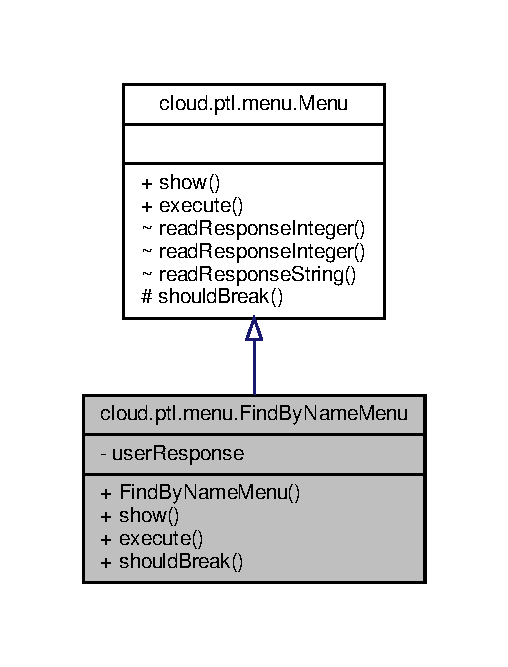
\includegraphics[width=244pt]{classcloud_1_1ptl_1_1menu_1_1FindByNameMenu__inherit__graph}
\end{center}
\end{figure}


Collaboration diagram for cloud.\+ptl.\+menu.\+Find\+By\+Name\+Menu\+:
\nopagebreak
\begin{figure}[H]
\begin{center}
\leavevmode
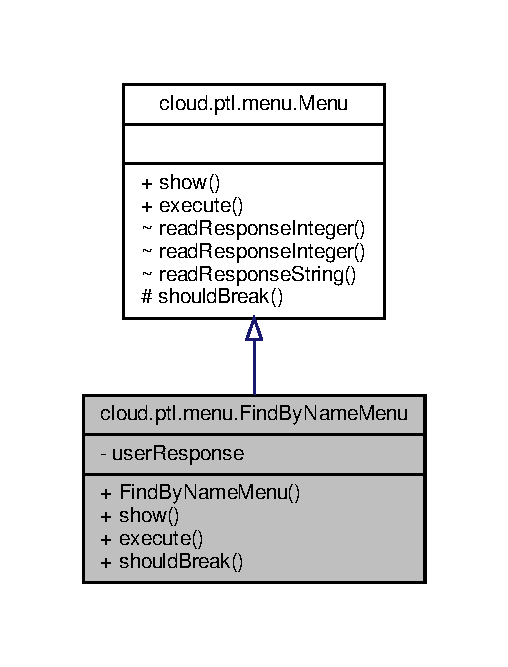
\includegraphics[width=244pt]{classcloud_1_1ptl_1_1menu_1_1FindByNameMenu__coll__graph}
\end{center}
\end{figure}
\subsection*{Public Member Functions}
\begin{DoxyCompactItemize}
\item 
\mbox{\Hypertarget{classcloud_1_1ptl_1_1menu_1_1FindByNameMenu_a55d24427391d7341248eee0d668cef73}\label{classcloud_1_1ptl_1_1menu_1_1FindByNameMenu_a55d24427391d7341248eee0d668cef73}} 
void {\bfseries show} ()
\item 
\mbox{\Hypertarget{classcloud_1_1ptl_1_1menu_1_1FindByNameMenu_ab1f6f91ed991a1c65da41e45ee5be066}\label{classcloud_1_1ptl_1_1menu_1_1FindByNameMenu_ab1f6f91ed991a1c65da41e45ee5be066}} 
void {\bfseries execute} ()
\item 
\mbox{\Hypertarget{classcloud_1_1ptl_1_1menu_1_1FindByNameMenu_a91da30bf29cf692109de3e23391a7c73}\label{classcloud_1_1ptl_1_1menu_1_1FindByNameMenu_a91da30bf29cf692109de3e23391a7c73}} 
Boolean {\bfseries should\+Break} ()
\end{DoxyCompactItemize}
\subsection*{Private Attributes}
\begin{DoxyCompactItemize}
\item 
\mbox{\Hypertarget{classcloud_1_1ptl_1_1menu_1_1FindByNameMenu_a332e611bd46ff34cd1b6e9dd935f7f65}\label{classcloud_1_1ptl_1_1menu_1_1FindByNameMenu_a332e611bd46ff34cd1b6e9dd935f7f65}} 
String {\bfseries user\+Response}
\end{DoxyCompactItemize}
\subsection*{Additional Inherited Members}


The documentation for this class was generated from the following file\+:\begin{DoxyCompactItemize}
\item 
src/main/java/cloud/ptl/menu/Find\+By\+Name\+Menu.\+java\end{DoxyCompactItemize}

\hypertarget{classcloud_1_1ptl_1_1menu_1_1FindBySurnameMenu}{}\section{cloud.\+ptl.\+menu.\+Find\+By\+Surname\+Menu Class Reference}
\label{classcloud_1_1ptl_1_1menu_1_1FindBySurnameMenu}\index{cloud.\+ptl.\+menu.\+Find\+By\+Surname\+Menu@{cloud.\+ptl.\+menu.\+Find\+By\+Surname\+Menu}}


Inheritance diagram for cloud.\+ptl.\+menu.\+Find\+By\+Surname\+Menu\+:
\nopagebreak
\begin{figure}[H]
\begin{center}
\leavevmode
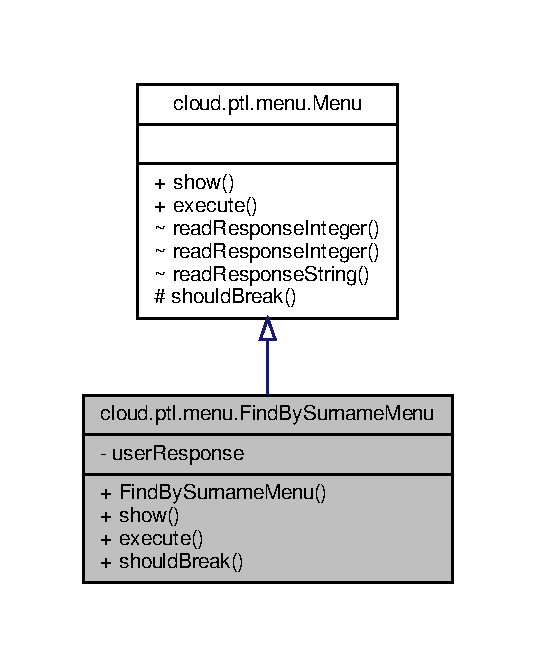
\includegraphics[width=257pt]{classcloud_1_1ptl_1_1menu_1_1FindBySurnameMenu__inherit__graph}
\end{center}
\end{figure}


Collaboration diagram for cloud.\+ptl.\+menu.\+Find\+By\+Surname\+Menu\+:
\nopagebreak
\begin{figure}[H]
\begin{center}
\leavevmode
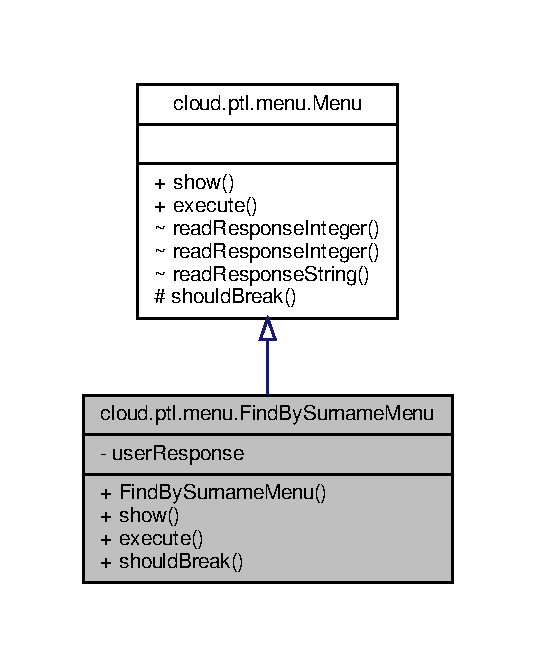
\includegraphics[width=257pt]{classcloud_1_1ptl_1_1menu_1_1FindBySurnameMenu__coll__graph}
\end{center}
\end{figure}
\subsection*{Public Member Functions}
\begin{DoxyCompactItemize}
\item 
\mbox{\Hypertarget{classcloud_1_1ptl_1_1menu_1_1FindBySurnameMenu_a3ceaf3ae4f0ab91483e0de9687928f80}\label{classcloud_1_1ptl_1_1menu_1_1FindBySurnameMenu_a3ceaf3ae4f0ab91483e0de9687928f80}} 
void {\bfseries show} ()
\item 
\mbox{\Hypertarget{classcloud_1_1ptl_1_1menu_1_1FindBySurnameMenu_a10f90fb3dab435801b6d7f0e66536d01}\label{classcloud_1_1ptl_1_1menu_1_1FindBySurnameMenu_a10f90fb3dab435801b6d7f0e66536d01}} 
void {\bfseries execute} ()
\item 
\mbox{\Hypertarget{classcloud_1_1ptl_1_1menu_1_1FindBySurnameMenu_a72d322ef1d72a120c2baa21a50adb03b}\label{classcloud_1_1ptl_1_1menu_1_1FindBySurnameMenu_a72d322ef1d72a120c2baa21a50adb03b}} 
Boolean {\bfseries should\+Break} ()
\end{DoxyCompactItemize}
\subsection*{Private Attributes}
\begin{DoxyCompactItemize}
\item 
\mbox{\Hypertarget{classcloud_1_1ptl_1_1menu_1_1FindBySurnameMenu_aaa1d62ad4db1b0a1c1a256166ca0d590}\label{classcloud_1_1ptl_1_1menu_1_1FindBySurnameMenu_aaa1d62ad4db1b0a1c1a256166ca0d590}} 
String {\bfseries user\+Response}
\end{DoxyCompactItemize}
\subsection*{Additional Inherited Members}


The documentation for this class was generated from the following file\+:\begin{DoxyCompactItemize}
\item 
src/main/java/cloud/ptl/menu/Find\+By\+Surname\+Menu.\+java\end{DoxyCompactItemize}

\hypertarget{classcloud_1_1ptl_1_1menu_1_1MainMenu}{}\section{cloud.\+ptl.\+menu.\+Main\+Menu Class Reference}
\label{classcloud_1_1ptl_1_1menu_1_1MainMenu}\index{cloud.\+ptl.\+menu.\+Main\+Menu@{cloud.\+ptl.\+menu.\+Main\+Menu}}


Inheritance diagram for cloud.\+ptl.\+menu.\+Main\+Menu\+:
\nopagebreak
\begin{figure}[H]
\begin{center}
\leavevmode
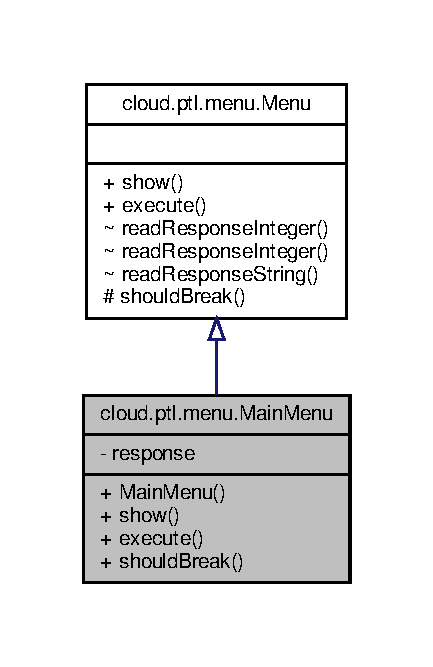
\includegraphics[width=208pt]{classcloud_1_1ptl_1_1menu_1_1MainMenu__inherit__graph}
\end{center}
\end{figure}


Collaboration diagram for cloud.\+ptl.\+menu.\+Main\+Menu\+:
\nopagebreak
\begin{figure}[H]
\begin{center}
\leavevmode
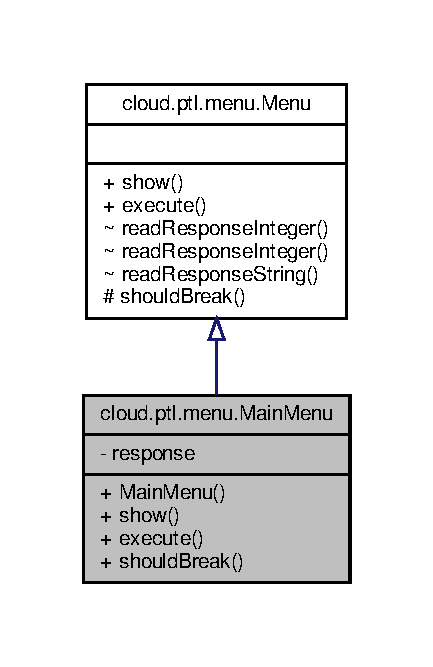
\includegraphics[width=208pt]{classcloud_1_1ptl_1_1menu_1_1MainMenu__coll__graph}
\end{center}
\end{figure}
\subsection*{Public Member Functions}
\begin{DoxyCompactItemize}
\item 
\mbox{\Hypertarget{classcloud_1_1ptl_1_1menu_1_1MainMenu_a9ec09bf872d3cf06cf8f923ff0f31474}\label{classcloud_1_1ptl_1_1menu_1_1MainMenu_a9ec09bf872d3cf06cf8f923ff0f31474}} 
void {\bfseries show} ()
\item 
\mbox{\Hypertarget{classcloud_1_1ptl_1_1menu_1_1MainMenu_ad4f6a2488523d99f0c2c8d644c4cbed1}\label{classcloud_1_1ptl_1_1menu_1_1MainMenu_ad4f6a2488523d99f0c2c8d644c4cbed1}} 
void {\bfseries execute} ()
\item 
\mbox{\Hypertarget{classcloud_1_1ptl_1_1menu_1_1MainMenu_ab8fc2592cbd3a71cc8dfc283d3cb5ddb}\label{classcloud_1_1ptl_1_1menu_1_1MainMenu_ab8fc2592cbd3a71cc8dfc283d3cb5ddb}} 
Boolean {\bfseries should\+Break} ()
\end{DoxyCompactItemize}
\subsection*{Private Attributes}
\begin{DoxyCompactItemize}
\item 
\mbox{\Hypertarget{classcloud_1_1ptl_1_1menu_1_1MainMenu_aa6233cbf30f22d819279452ccf0c812c}\label{classcloud_1_1ptl_1_1menu_1_1MainMenu_aa6233cbf30f22d819279452ccf0c812c}} 
Integer {\bfseries response}
\end{DoxyCompactItemize}
\subsection*{Additional Inherited Members}


The documentation for this class was generated from the following file\+:\begin{DoxyCompactItemize}
\item 
src/main/java/cloud/ptl/menu/Main\+Menu.\+java\end{DoxyCompactItemize}

\hypertarget{classcloud_1_1ptl_1_1menu_1_1Menu}{}\section{cloud.\+ptl.\+menu.\+Menu Class Reference}
\label{classcloud_1_1ptl_1_1menu_1_1Menu}\index{cloud.\+ptl.\+menu.\+Menu@{cloud.\+ptl.\+menu.\+Menu}}


Inheritance diagram for cloud.\+ptl.\+menu.\+Menu\+:
\nopagebreak
\begin{figure}[H]
\begin{center}
\leavevmode
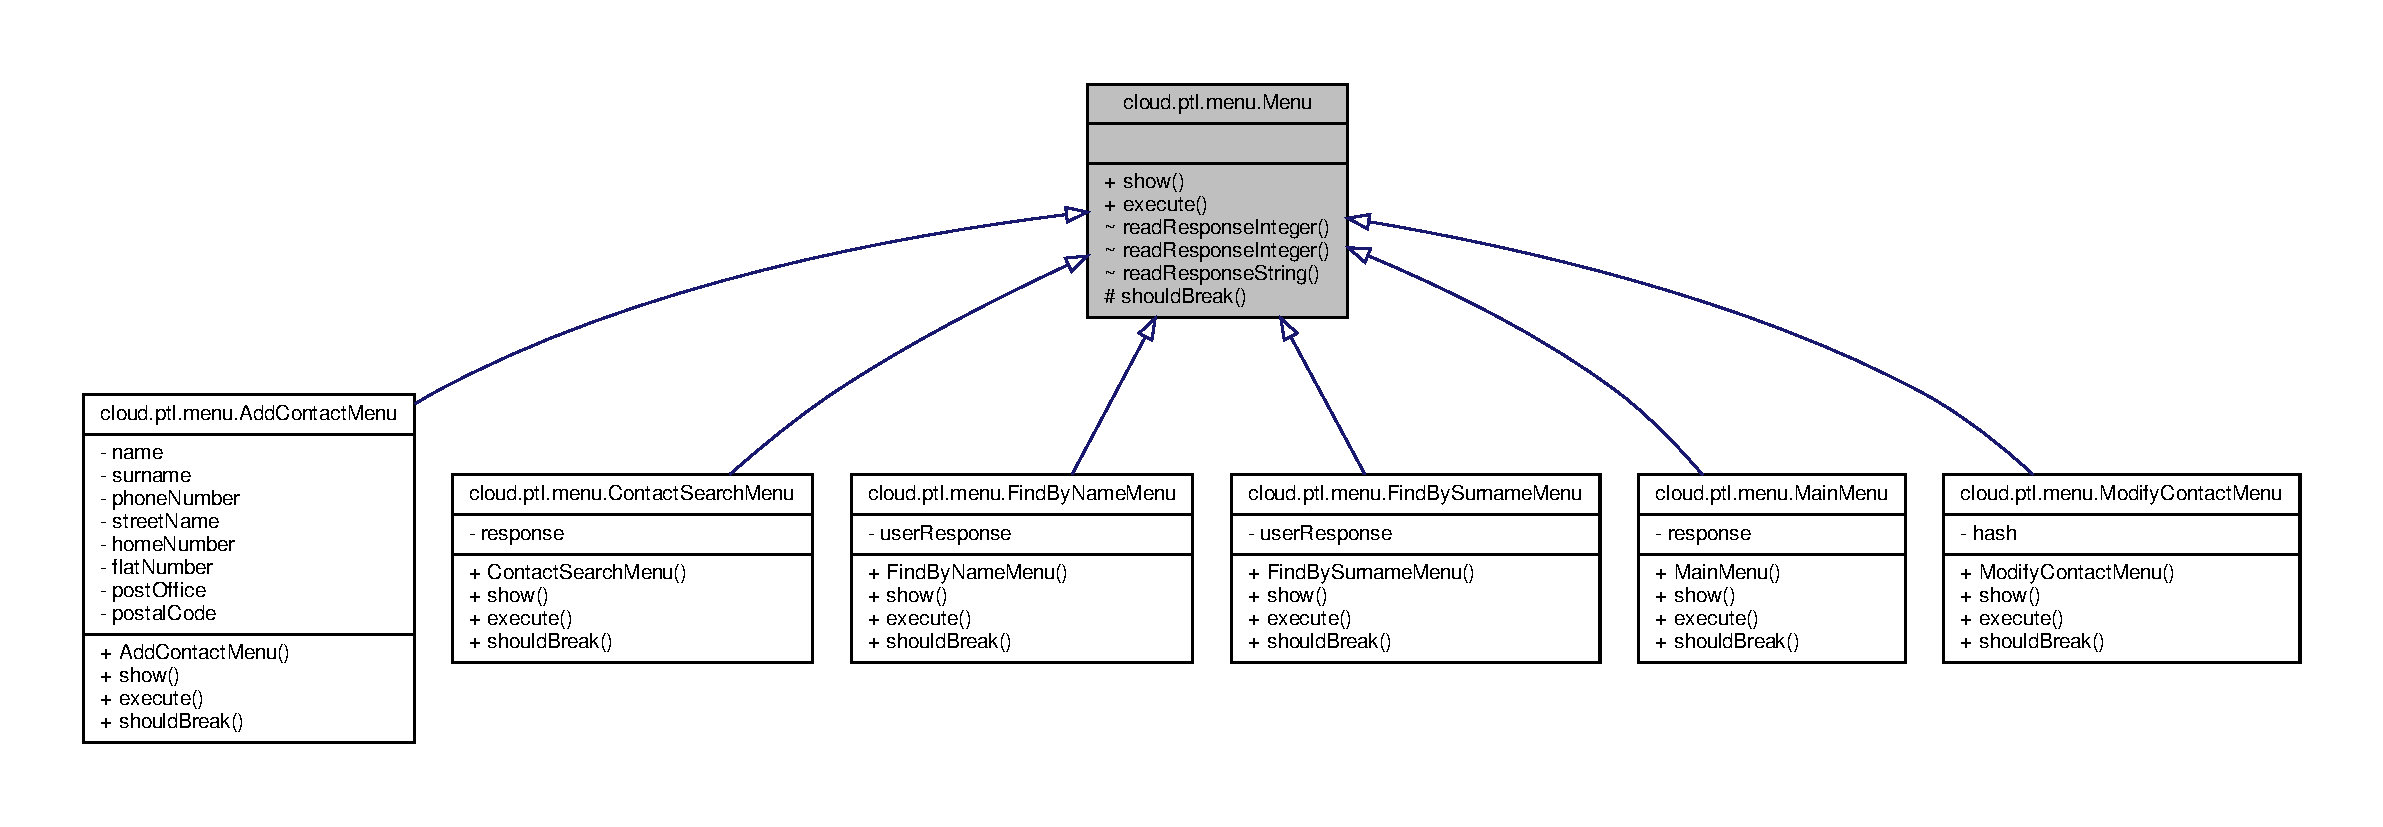
\includegraphics[width=350pt]{classcloud_1_1ptl_1_1menu_1_1Menu__inherit__graph}
\end{center}
\end{figure}


Collaboration diagram for cloud.\+ptl.\+menu.\+Menu\+:
\nopagebreak
\begin{figure}[H]
\begin{center}
\leavevmode
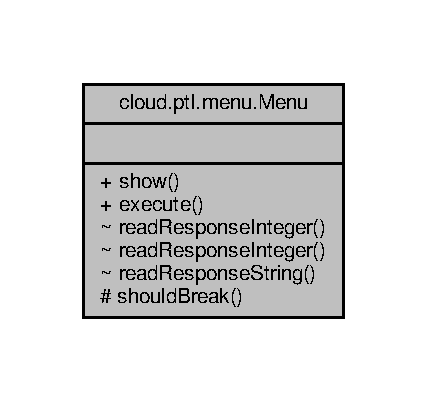
\includegraphics[width=205pt]{classcloud_1_1ptl_1_1menu_1_1Menu__coll__graph}
\end{center}
\end{figure}
\subsection*{Public Member Functions}
\begin{DoxyCompactItemize}
\item 
\mbox{\Hypertarget{classcloud_1_1ptl_1_1menu_1_1Menu_a8fd769cd1ee8efca8a90433ffce38212}\label{classcloud_1_1ptl_1_1menu_1_1Menu_a8fd769cd1ee8efca8a90433ffce38212}} 
abstract void {\bfseries show} ()
\item 
\mbox{\Hypertarget{classcloud_1_1ptl_1_1menu_1_1Menu_a7078af5d8e55c04efaf15b00fcf07906}\label{classcloud_1_1ptl_1_1menu_1_1Menu_a7078af5d8e55c04efaf15b00fcf07906}} 
abstract void {\bfseries execute} ()
\end{DoxyCompactItemize}
\subsection*{Protected Member Functions}
\begin{DoxyCompactItemize}
\item 
\mbox{\Hypertarget{classcloud_1_1ptl_1_1menu_1_1Menu_ad6022bbd37ee52964b2327b593902666}\label{classcloud_1_1ptl_1_1menu_1_1Menu_ad6022bbd37ee52964b2327b593902666}} 
abstract Boolean {\bfseries should\+Break} ()
\end{DoxyCompactItemize}


The documentation for this class was generated from the following file\+:\begin{DoxyCompactItemize}
\item 
src/main/java/cloud/ptl/menu/Menu.\+java\end{DoxyCompactItemize}

\hypertarget{classcloud_1_1ptl_1_1menu_1_1ModifyContactMenu}{}\section{cloud.\+ptl.\+menu.\+Modify\+Contact\+Menu Class Reference}
\label{classcloud_1_1ptl_1_1menu_1_1ModifyContactMenu}\index{cloud.\+ptl.\+menu.\+Modify\+Contact\+Menu@{cloud.\+ptl.\+menu.\+Modify\+Contact\+Menu}}


Inheritance diagram for cloud.\+ptl.\+menu.\+Modify\+Contact\+Menu\+:
\nopagebreak
\begin{figure}[H]
\begin{center}
\leavevmode
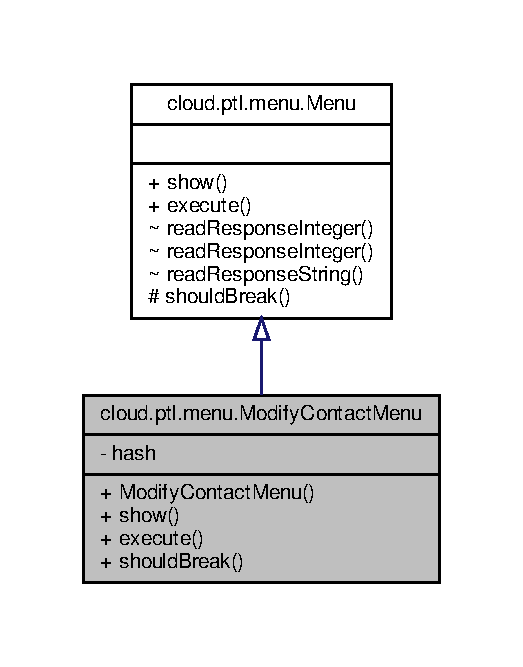
\includegraphics[width=251pt]{classcloud_1_1ptl_1_1menu_1_1ModifyContactMenu__inherit__graph}
\end{center}
\end{figure}


Collaboration diagram for cloud.\+ptl.\+menu.\+Modify\+Contact\+Menu\+:
\nopagebreak
\begin{figure}[H]
\begin{center}
\leavevmode
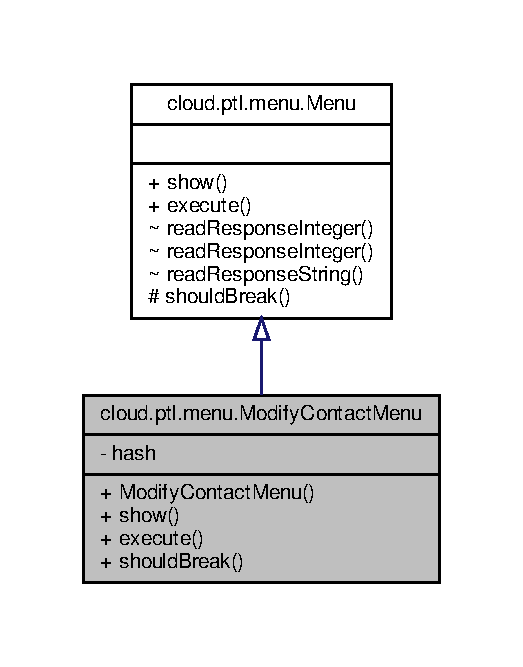
\includegraphics[width=251pt]{classcloud_1_1ptl_1_1menu_1_1ModifyContactMenu__coll__graph}
\end{center}
\end{figure}
\subsection*{Public Member Functions}
\begin{DoxyCompactItemize}
\item 
\mbox{\Hypertarget{classcloud_1_1ptl_1_1menu_1_1ModifyContactMenu_ad0d13c849aed2d47ad320847a768d0db}\label{classcloud_1_1ptl_1_1menu_1_1ModifyContactMenu_ad0d13c849aed2d47ad320847a768d0db}} 
void {\bfseries show} ()
\item 
\mbox{\Hypertarget{classcloud_1_1ptl_1_1menu_1_1ModifyContactMenu_a9a1dc878f82cdfdac1badeabf6e5a8bc}\label{classcloud_1_1ptl_1_1menu_1_1ModifyContactMenu_a9a1dc878f82cdfdac1badeabf6e5a8bc}} 
void {\bfseries execute} ()
\item 
\mbox{\Hypertarget{classcloud_1_1ptl_1_1menu_1_1ModifyContactMenu_a12ab2eb24fa364668c4800bd0693f59b}\label{classcloud_1_1ptl_1_1menu_1_1ModifyContactMenu_a12ab2eb24fa364668c4800bd0693f59b}} 
Boolean {\bfseries should\+Break} ()
\end{DoxyCompactItemize}
\subsection*{Private Attributes}
\begin{DoxyCompactItemize}
\item 
\mbox{\Hypertarget{classcloud_1_1ptl_1_1menu_1_1ModifyContactMenu_a1b2c93a68eda3ac1500c91b0212fc042}\label{classcloud_1_1ptl_1_1menu_1_1ModifyContactMenu_a1b2c93a68eda3ac1500c91b0212fc042}} 
String {\bfseries hash}
\end{DoxyCompactItemize}
\subsection*{Additional Inherited Members}


The documentation for this class was generated from the following file\+:\begin{DoxyCompactItemize}
\item 
src/main/java/cloud/ptl/menu/Modify\+Contact\+Menu.\+java\end{DoxyCompactItemize}

%--- End generated contents ---

% Index
\backmatter
\newpage
\phantomsection
\clearemptydoublepage
\addcontentsline{toc}{chapter}{Index}
\printindex

\end{document}
